%%%%%%%%%%%%%%%%%%%%%%%%%%%%%%%%%%%%%%%%%%%%%%%%%%%%%%%%%%%%%%%%%%%%%%%%%%%%%%%
% CASE STUDY TEMPLATE - Programming and Problem Solving
% Author: Brendan Shea, PhD
% Course: Programming and Problem Solving
% Rochester Community and Technical College
%%%%%%%%%%%%%%%%%%%%%%%%%%%%%%%%%%%%%%%%%%%%%%%%%%%%%%%%%%%%%%%%%%%%%%%%%%%%%%%

\documentclass[11pt,letterpaper]{article}

%---------- PACKAGES ----------%
\usepackage[margin=1in, headheight=22pt]{geometry}
\usepackage[T1]{fontenc}
\usepackage{xcolor}
\usepackage{tcolorbox}
\usepackage{graphicx}
\usepackage{titlesec}
\usepackage{enumitem}
\usepackage{fancyhdr}
\usepackage{listings}
\usepackage{hyperref}
\usepackage{multicol}
\usepackage{booktabs}
\usepackage{tikz}
\usepackage{float}
\usepackage{amssymb}
\usepackage{amsmath}
\usepackage{pifont}

% TikZ libraries
\usetikzlibrary{shapes.geometric, arrows.meta, positioning, calc, backgrounds, fit, matrix, decorations.pathreplacing}

% Load tcolorbox libraries
\tcbuselibrary{skins,breakable,listings,listingsutf8}

%---------- COLOR DEFINITIONS ----------%
\definecolor{csprimary}{HTML}{2C3E50}
\definecolor{cssecondary}{HTML}{E74C3C}
\definecolor{cstertiary}{HTML}{3498DB}
\definecolor{csaccent}{HTML}{27AE60}
\definecolor{cswarm}{HTML}{F39C12}
\definecolor{cslight}{HTML}{ECF0F1}
\definecolor{csdark}{HTML}{1A252F}

% Syntax highlighting colors
\definecolor{codegreen}{HTML}{27AE60}
\definecolor{codepurple}{HTML}{9B59B6}
\definecolor{codeorange}{HTML}{E67E22}
\definecolor{codeblue}{HTML}{3498DB}
\definecolor{codegray}{HTML}{95A5A6}
\definecolor{codestring}{HTML}{E74C3C}
\definecolor{codebg}{HTML}{1E2A38}

%---------- CASE STUDY METADATA ----------%
\newcommand{\cstitle}{Famous Functions}
\newcommand{\cssubtitle}{From Pythagoras to Binary Search}
\newcommand{\csauthor}{Brendan Shea, PhD}
\newcommand{\cscourse}{Programming and Problem Solving}
\newcommand{\csinstitution}{Rochester Community and Technical College}
\newcommand{\csdate}{\today}

%---------- LISTINGS CONFIGURATION ----------%
\lstdefinestyle{basestyle}{
    backgroundcolor=\color{codebg},
    basicstyle=\ttfamily\small\color{white},
    breakatwhitespace=false,
    breaklines=true,
    captionpos=b,
    keepspaces=true,
    showspaces=false,
    showstringspaces=false,
    showtabs=false,
    tabsize=4,
    frame=none,
    xleftmargin=4mm,
    xrightmargin=4mm,
    aboveskip=0pt,
    belowskip=0pt,
}

\lstdefinestyle{javastyle}{
    style=basestyle,
    language=Java,
    keywordstyle=\color{codeblue}\bfseries,
    commentstyle=\color{codegray}\itshape,
    stringstyle=\color{codestring},
    morekeywords={String, Scanner, System, var, boolean, Math},
}

%---------- CUSTOM ENVIRONMENTS ----------%
\newcommand{\keyterm}[1]{\textbf{\textcolor{cssecondary}{#1}}}

\newtcolorbox{conceptbox}[1][]{
    enhanced,
    colback=cslight,
    colframe=csprimary,
    fonttitle=\bfseries\color{white},
    title=#1,
    attach boxed title to top left={yshift=-2mm, xshift=5mm},
    boxed title style={colback=csprimary},
    breakable
}

\newtcolorbox{historybox}[1][]{
    enhanced,
    colback=codepurple!8,
    colframe=codepurple,
    fonttitle=\bfseries\color{white},
    title=#1,
    attach boxed title to top left={yshift=-2mm, xshift=5mm},
    boxed title style={colback=codepurple},
    breakable
}

\newtcolorbox{mathbox}[1][]{
    enhanced,
    colback=cstertiary!8,
    colframe=cstertiary,
    fonttitle=\bfseries\color{white},
    title=#1,
    attach boxed title to top left={yshift=-2mm, xshift=5mm},
    boxed title style={colback=cstertiary},
    breakable
}

\newtcblisting{javacode}[1][]{
    enhanced,
    colback=codebg,
    colframe=csaccent,
    colupper=white,
    fonttitle=\bfseries\color{white},
    title=#1,
    attach boxed title to top left={yshift=-2mm, xshift=5mm},
    boxed title style={colback=csaccent},
    left=0mm, right=0mm, top=2mm, bottom=2mm,
    boxrule=1pt,
    breakable,
    pad at break=2mm,
    listing only,
    listing options={style=javastyle}
}

\newtcolorbox{questionbox}{
    enhanced,
    colback=cswarm!10,
    colframe=cswarm,
    fonttitle=\bfseries\color{white},
    title=Discussion Questions,
    attach boxed title to top center={yshift=-2mm},
    boxed title style={colback=cswarm},
    breakable
}

\newtcolorbox{glossarybox}{
    enhanced,
    colback=cslight,
    colframe=csprimary,
    fonttitle=\bfseries\color{white},
    title=Glossary of Key Terms,
    attach boxed title to top center={yshift=-2mm},
    boxed title style={colback=csprimary},
    breakable
}

%---------- HEADER/FOOTER ----------%
\pagestyle{fancy}
\fancyhf{}
\fancyhead[L]{\small\textcolor{csprimary}{\cscourse}}
\fancyhead[R]{\small\textcolor{csprimary}{Case Study}}
\fancyfoot[C]{\thepage}
\renewcommand{\headrulewidth}{0.4pt}
\renewcommand{\headrule}{\hbox to\headwidth{\color{csprimary}\leaders\hrule height \headrulewidth\hfill}}

%---------- SECTION FORMATTING ----------%
\titleformat{\section}
    {\Large\bfseries\color{csprimary}}
    {\thesection}{1em}{}[\color{cssecondary}\titlerule]
    
\titleformat{\subsection}
    {\large\bfseries\color{cstertiary}}
    {\thesubsection}{1em}{}

%---------- HYPERLINK SETTINGS ----------%
\hypersetup{
    colorlinks=true,
    linkcolor=cstertiary,
    urlcolor=cstertiary
}

%%%%%%%%%%%%%%%%%%%%%%%%%%%%%%%%%%%%%%%%%%%%%%%%%%%%%%%%%%%%%%%%%%%%%%%%%%%%%%%
\begin{document}

%---------- TITLE BLOCK ----------%
\begin{tcolorbox}[
    enhanced,
    colback=csprimary,
    colframe=csprimary,
    arc=0mm,
    left=10mm, right=10mm, top=8mm, bottom=8mm
]
\begin{center}
    {\huge\bfseries\color{white}\cstitle}\\[3mm]
    {\Large\color{cslight}\cssubtitle}\\[5mm]
    \textcolor{cssecondary}{\rule{0.5\textwidth}{1pt}}\\[5mm]
    {\large\color{white}\csauthor}\\[2mm]
    {\normalsize\color{cslight}\cscourse\ $\bullet$ \csinstitution}
\end{center}
\end{tcolorbox}

\vspace{5mm}

%---------- INTRODUCTION ----------%
\section*{Introduction}

Every programmer stands on the shoulders of giants. The functions we write today---whether calculating distances, searching through data, or solving equations---have roots stretching back thousands of years. Ancient mathematicians discovered the formulas; pioneering computer scientists figured out how to express them as algorithms; and now you're learning to implement them in Java.

This case study explores several ``famous functions'': mathematical and computational procedures so useful that they've been implemented billions of times across every programming language. Along the way, you'll learn not just \textit{how} to write functions, but \textit{why} functions are structured the way they are, and how to design your own.

\begin{conceptbox}[What You'll Learn]
\begin{itemize}[leftmargin=*, itemsep=2pt]
    \item What functions are and why they're fundamental to programming
    \item The history and mathematics behind classic algorithms
    \item How to implement the Pythagorean theorem, quadratic formula, factorial, and search algorithms
    \item Principles for designing, implementing, and testing your own functions
\end{itemize}
\end{conceptbox}

%---------- WHAT ARE FUNCTIONS ----------%
\section{What Are Functions?}

A \keyterm{function} (also called a \textit{method} in Java) is a reusable block of code that performs a specific task. You give it inputs, it does some work, and it returns an output. Think of a function like a machine: raw materials go in, a product comes out.

\begin{center}
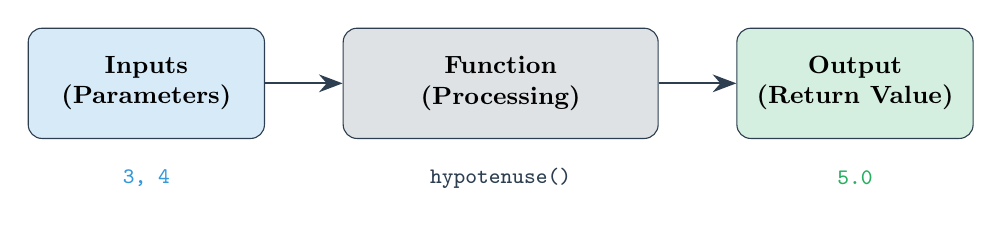
\begin{tikzpicture}[
    box/.style={rectangle, rounded corners=5pt, draw=csprimary, fill=#1, minimum width=30mm, minimum height=14mm, font=\small\bfseries, align=center},
    arrow/.style={-{Stealth[length=3mm]}, thick, color=csprimary}
]

\node[box=cstertiary!20] (input) at (0,0) {Inputs\\(Parameters)};
\node[box=csprimary!15, minimum width=40mm] (func) at (4.5,0) {Function\\(Processing)};
\node[box=csaccent!20] (output) at (9,0) {Output\\(Return Value)};

\draw[arrow] (input) -- (func);
\draw[arrow] (func) -- (output);

% Example below
\node[font=\footnotesize\ttfamily, color=cstertiary] at (0,-1.2) {3, 4};
\node[font=\footnotesize\ttfamily, color=csprimary] at (4.5,-1.2) {hypotenuse()};
\node[font=\footnotesize\ttfamily, color=csaccent] at (9,-1.2) {5.0};

\end{tikzpicture}
\end{center}

Why do we use functions? Three crucial reasons:

\textbf{Reusability.} Once you write a function to calculate a hypotenuse, you can use it anywhere in your program---or in future programs---without rewriting the logic. Write once, use forever.

\textbf{Abstraction.} Functions let you hide complexity. When you call \texttt{Math.sqrt(x)}, you don't need to know \textit{how} the square root is calculated. You just trust that it works. This lets you think at higher levels.

\textbf{Organization.} Breaking a program into functions makes it easier to understand, test, and debug. Each function has one job, and you can verify that job works correctly in isolation.

\subsection{Anatomy of a Java Function}

Let's examine the parts of a function:

\begin{javacode}[Anatomy of a Function]
//  return type    name        parameters
//      |           |              |
//      v           v              v
    public static double hypotenuse(double a, double b) {
        double cSquared = a * a + b * b;  // body: the work
        return Math.sqrt(cSquared);       // return statement
    }
\end{javacode}

The \keyterm{return type} (\texttt{double}) declares what kind of value the function produces. The \keyterm{parameters} (\texttt{double a, double b}) are the inputs the function expects. The \keyterm{body} contains the actual code that does the work. The \keyterm{return statement} sends the result back to whoever called the function.

When you call this function with \texttt{hypotenuse(3, 4)}, Java substitutes 3 for \texttt{a} and 4 for \texttt{b}, executes the body, and gives you back 5.0.

%---------- PYTHAGOREAN THEOREM ----------%
\section{The Pythagorean Theorem}

\begin{historybox}[Pythagoras of Samos (c.\ 570--495 BCE)]
Pythagoras was a Greek philosopher and mathematician who founded a religious movement based on mathematics. His followers, the Pythagoreans, believed that numbers were the ultimate reality underlying the universe. While Pythagoras himself may not have discovered the theorem bearing his name---Babylonian mathematicians knew it a thousand years earlier---his school provided the first known proof, elevating it from an observed pattern to a demonstrated truth.
\end{historybox}

The \keyterm{Pythagorean theorem} states that in a right triangle, the square of the hypotenuse (the side opposite the right angle) equals the sum of the squares of the other two sides:

\begin{mathbox}[The Formula]
\[ a^2 + b^2 = c^2 \]
Therefore: $c = \sqrt{a^2 + b^2}$
\end{mathbox}

This formula is everywhere: calculating distances on maps, determining screen dimensions, physics simulations, game development, and anywhere else geometry matters. Let's implement it:

\begin{javacode}[Pythagorean Theorem in Java]
/**
 * Calculates the length of the hypotenuse of a right triangle.
 * @param a length of one leg
 * @param b length of other leg
 * @return length of the hypotenuse
 */
public static double hypotenuse(double a, double b) {
    return Math.sqrt(a * a + b * b);
}

// Example usage:
double distance = hypotenuse(3, 4);  // returns 5.0
\end{javacode}

\begin{center}
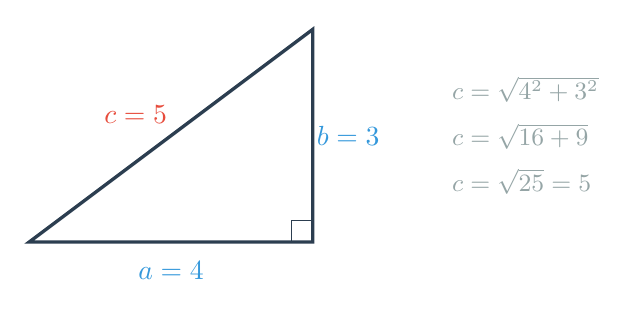
\begin{tikzpicture}[scale=0.9]
    % Triangle
    \draw[very thick, csprimary] (0,0) -- (4,0) -- (4,3) -- cycle;
    
    % Right angle mark
    \draw[csprimary] (3.7,0) -- (3.7,0.3) -- (4,0.3);
    
    % Labels
    \node[font=\bfseries, color=cstertiary] at (2,-0.4) {$a = 4$};
    \node[font=\bfseries, color=cstertiary] at (4.5,1.5) {$b = 3$};
    \node[font=\bfseries, color=cssecondary] at (1.5,1.8) {$c = 5$};
    
    % Formula
    \node[font=\small, color=codegray, align=left] at (7,1.5) {$c = \sqrt{4^2 + 3^2}$\\[2mm]$c = \sqrt{16 + 9}$\\[2mm]$c = \sqrt{25} = 5$};
\end{tikzpicture}
\end{center}

Notice the \keyterm{Javadoc comment} (the comment starting with \texttt{/**}). This documents what the function does, what parameters it expects, and what it returns. Good documentation is part of writing good functions.

%---------- QUADRATIC FORMULA ----------%
\section{The Quadratic Formula}

\begin{historybox}[From Babylon to al-Khwarizmi]
Babylonian mathematicians solved quadratic equations around 2000 BCE, but only for specific cases and without a general formula. The Persian mathematician Muhammad ibn Musa al-Khwarizmi (c.\ 780--850 CE) wrote a systematic treatment of equation-solving in his book \textit{Al-Kitab al-mukhtasar}. His name gave us the word ``algorithm,'' and his methods evolved into the quadratic formula we use today.
\end{historybox}

A \keyterm{quadratic equation} has the form $ax^2 + bx + c = 0$. The quadratic formula finds the values of $x$ that satisfy this equation:

\begin{mathbox}[The Quadratic Formula]
\[ x = \frac{-b \pm \sqrt{b^2 - 4ac}}{2a} \]
The expression $b^2 - 4ac$ is called the \textbf{discriminant}.
\end{mathbox}

The \keyterm{discriminant} tells us how many solutions exist: if it's positive, there are two real solutions; if zero, one solution; if negative, no real solutions (only complex numbers).

Implementing this in Java requires us to handle these cases:

\begin{javacode}[Quadratic Formula in Java]
/**
 * Solves ax^2 + bx + c = 0 and returns the solutions.
 * @return array of solutions (0, 1, or 2 elements)
 */
public static double[] solveQuadratic(double a, double b, double c) {
    double discriminant = b * b - 4 * a * c;
    
    if (discriminant < 0) {
        // No real solutions
        return new double[0];  // empty array
    } else if (discriminant == 0) {
        // One solution (repeated root)
        double x = -b / (2 * a);
        return new double[] { x };
    } else {
        // Two solutions
        double sqrtDisc = Math.sqrt(discriminant);
        double x1 = (-b + sqrtDisc) / (2 * a);
        double x2 = (-b - sqrtDisc) / (2 * a);
        return new double[] { x1, x2 };
    }
}

// Example: solve x^2 - 5x + 6 = 0
double[] roots = solveQuadratic(1, -5, 6);  // returns {3.0, 2.0}
\end{javacode}

This function returns an \textit{array} because the number of solutions varies. The function's design reflects the mathematical reality: sometimes there's no answer, sometimes one, sometimes two.

%---------- FACTORIAL ----------%
\section{The Factorial Function}

\begin{historybox}[Factorial Through History]
Factorial calculations appear in ancient Indian mathematics (the Jain text \textit{Anuyogadwara Sutra}, c.\ 200 BCE) in the context of counting permutations. The modern notation $n!$ was introduced by Christian Kramp in 1808. Factorials are fundamental to combinatorics (counting arrangements), probability theory, and appear unexpectedly in calculus through Taylor series.
\end{historybox}

The \keyterm{factorial} of a positive integer $n$, written $n!$, is the product of all positive integers from 1 to $n$:

\begin{mathbox}[Factorial Definition]
\[ n! = n \times (n-1) \times (n-2) \times \cdots \times 2 \times 1 \]
By convention, $0! = 1$.

Examples: $5! = 5 \times 4 \times 3 \times 2 \times 1 = 120$
\end{mathbox}

Factorial has a beautiful property: $n! = n \times (n-1)!$. This means we can define factorial in terms of itself---a technique called \keyterm{recursion}.

\begin{javacode}[Factorial: Iterative vs.\ Recursive]
// Iterative approach: use a loop
public static long factorialIterative(int n) {
    long result = 1;
    for (int i = 2; i <= n; i++) {
        result *= i;  // multiply result by each number
    }
    return result;
}

// Recursive approach: function calls itself
public static long factorialRecursive(int n) {
    if (n <= 1) {
        return 1;  // base case: 0! = 1! = 1
    } else {
        return n * factorialRecursive(n - 1);  // recursive case
    }
}
\end{javacode}

\begin{center}
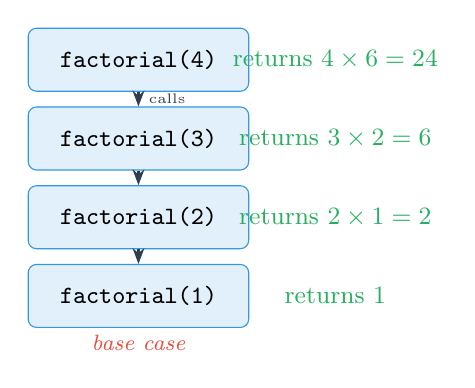
\begin{tikzpicture}[
    node distance=0.8cm,
    call/.style={rectangle, rounded corners=3pt, draw=cstertiary, fill=cstertiary!15, minimum width=28mm, minimum height=8mm, font=\small\ttfamily},
    arrow/.style={-{Stealth[length=2mm]}, thick, color=csprimary}
]

% Recursive calls going down
\node[call] (f4) at (0,0) {factorial(4)};
\node[call] (f3) at (0,-1) {factorial(3)};
\node[call] (f2) at (0,-2) {factorial(2)};
\node[call] (f1) at (0,-3) {factorial(1)};

\draw[arrow] (f4.south) -- (f3.north) node[midway, right, font=\tiny\color{codegray}] {calls};
\draw[arrow] (f3.south) -- (f2.north);
\draw[arrow] (f2.south) -- (f1.north);

% Return values going up
\node[font=\small\color{csaccent}] at (2.5,-3) {returns 1};
\node[font=\small\color{csaccent}] at (2.5,-2) {returns $2 \times 1 = 2$};
\node[font=\small\color{csaccent}] at (2.5,-1) {returns $3 \times 2 = 6$};
\node[font=\small\color{csaccent}] at (2.5,0) {returns $4 \times 6 = 24$};

% Base case label
\node[font=\footnotesize\itshape, color=cssecondary] at (0,-3.6) {base case};

\end{tikzpicture}
\end{center}

Every recursive function needs a \keyterm{base case}---a condition where it stops calling itself and returns a direct answer. Without a base case, the function would call itself forever (until your computer runs out of memory).

Note that we use \texttt{long} instead of \texttt{int} because factorials grow extremely fast. Even so, $21!$ exceeds what a \texttt{long} can hold!

%---------- LINEAR SEARCH ----------%
\section{Linear Search}

Now we move from mathematics to computer science. \keyterm{Searching}---finding a specific item in a collection---is one of computing's most fundamental operations. The simplest approach is \keyterm{linear search}: check each element one by one until you find what you're looking for.

\begin{javacode}[Linear Search]
/**
 * Searches for a target value in an array.
 * @return index of target, or -1 if not found
 */
public static int linearSearch(int[] array, int target) {
    for (int i = 0; i < array.length; i++) {
        if (array[i] == target) {
            return i;  // found it! return the index
        }
    }
    return -1;  // searched everything, not found
}

// Example:
int[] numbers = {4, 2, 7, 1, 9, 3};
int index = linearSearch(numbers, 7);  // returns 2
\end{javacode}

\begin{center}
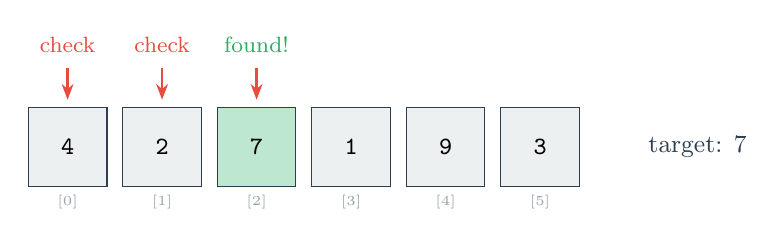
\begin{tikzpicture}[
    cell/.style={rectangle, draw=csprimary, fill=#1, minimum width=10mm, minimum height=10mm, font=\ttfamily\small},
    arrow/.style={-{Stealth[length=2mm]}, thick, color=cssecondary}
]

% Array cells
\node[cell=cslight] (c0) at (0,0) {4};
\node[cell=cslight] (c1) at (1.2,0) {2};
\node[cell=csaccent!30] (c2) at (2.4,0) {7};
\node[cell=cslight] (c3) at (3.6,0) {1};
\node[cell=cslight] (c4) at (4.8,0) {9};
\node[cell=cslight] (c5) at (6,0) {3};

% Indices
\node[font=\tiny\color{codegray}] at (0,-0.7) {[0]};
\node[font=\tiny\color{codegray}] at (1.2,-0.7) {[1]};
\node[font=\tiny\color{codegray}] at (2.4,-0.7) {[2]};
\node[font=\tiny\color{codegray}] at (3.6,-0.7) {[3]};
\node[font=\tiny\color{codegray}] at (4.8,-0.7) {[4]};
\node[font=\tiny\color{codegray}] at (6,-0.7) {[5]};

% Search arrows
\draw[arrow] (0,1) -- (0,0.6);
\draw[arrow] (1.2,1) -- (1.2,0.6);
\draw[arrow] (2.4,1) -- (2.4,0.6);

\node[font=\footnotesize\color{cssecondary}] at (0,1.3) {check};
\node[font=\footnotesize\color{cssecondary}] at (1.2,1.3) {check};
\node[font=\footnotesize\color{csaccent}] at (2.4,1.3) {found!};

% Target label
\node[font=\small, color=csprimary] at (8,0) {target: 7};

\end{tikzpicture}
\end{center}

Linear search is simple and works on any array, sorted or not. But it's slow for large collections: if you have a million elements, you might need to check all million. Computer scientists describe this as \keyterm{O(n)} or ``linear time''---the time grows proportionally with the input size.

%---------- BINARY SEARCH ----------%
\section{Binary Search}

\begin{historybox}[The Birth of Binary Search]
Binary search is ancient in concept---it's how you naturally search a dictionary or phone book. But implementing it correctly in code proved surprisingly tricky. Jon Bentley reported in his 1986 book \textit{Programming Pearls} that when he asked professional programmers to write binary search, 90\% got it wrong. The first bug-free published binary search appeared in 1962, sixteen years after the first description of the algorithm!
\end{historybox}

If the array is \textit{sorted}, we can do much better than linear search. \keyterm{Binary search} repeatedly divides the search space in half:

\begin{enumerate}[itemsep=2pt]
    \item Look at the middle element.
    \item If it's your target, you're done.
    \item If your target is smaller, search the left half.
    \item If your target is larger, search the right half.
    \item Repeat until found or the search space is empty.
\end{enumerate}

\begin{javacode}[Binary Search]
/**
 * Searches for target in a SORTED array.
 * @return index of target, or -1 if not found
 */
public static int binarySearch(int[] array, int target) {
    int left = 0;
    int right = array.length - 1;
    
    while (left <= right) {
        int mid = left + (right - left) / 2;  // find middle
        
        if (array[mid] == target) {
            return mid;  // found it!
        } else if (array[mid] < target) {
            left = mid + 1;  // target is in right half
        } else {
            right = mid - 1;  // target is in left half
        }
    }
    return -1;  // not found
}
\end{javacode}

\begin{center}
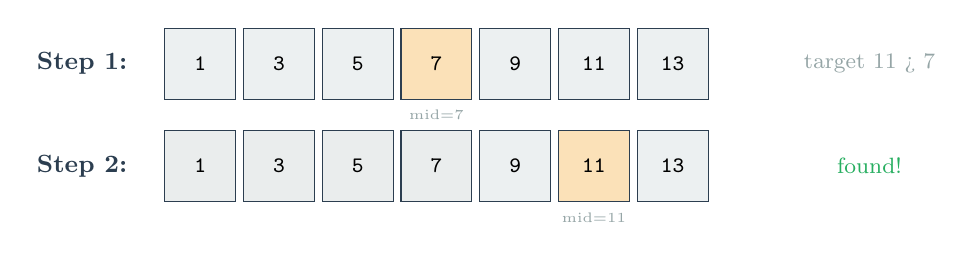
\begin{tikzpicture}[
    cell/.style={rectangle, draw=csprimary, fill=#1, minimum width=9mm, minimum height=9mm, font=\ttfamily\footnotesize},
]

% Step 1
\node[font=\small\bfseries, color=csprimary] at (-1.5,0) {Step 1:};
\foreach \i/\v/\c in {0/1/cslight, 1/3/cslight, 2/5/cslight, 3/7/cswarm!30, 4/9/cslight, 5/11/cslight, 6/13/cslight} {
    \node[cell=\c] at (\i*1.0,0) {\v};
}
\node[font=\tiny\color{codegray}] at (3,-0.65) {mid=7};
\node[font=\footnotesize\color{codegray}] at (8.5,0) {target 11 > 7};

% Step 2
\node[font=\small\bfseries, color=csprimary] at (-1.5,-1.3) {Step 2:};
\foreach \i/\v/\c in {0/1/codegray!20, 1/3/codegray!20, 2/5/codegray!20, 3/7/codegray!20, 4/9/cslight, 5/11/cswarm!30, 6/13/cslight} {
    \node[cell=\c] at (\i*1.0,-1.3) {\v};
}
\node[font=\tiny\color{codegray}] at (5,-1.95) {mid=11};
\node[font=\footnotesize\color{csaccent}] at (8.5,-1.3) {found!};

\end{tikzpicture}
\end{center}

Binary search is \keyterm{O(log n)}---logarithmic time. For a million elements, linear search might need a million comparisons; binary search needs at most 20. For a billion elements: 30 comparisons. This dramatic improvement is why sorting data is often worthwhile---it enables fast searching.

%---------- DESIGNING FUNCTIONS ----------%
\section{Designing Your Own Functions}

Now that you've seen famous functions, how do you create your own? Here's a systematic approach:

\subsection{Step 1: Define the Contract}

Before writing code, answer these questions:
\begin{itemize}[itemsep=2pt]
    \item What does this function do? (One clear task)
    \item What inputs does it need? (Parameters and their types)
    \item What output does it produce? (Return type)
    \item What are the edge cases? (Empty arrays, zero, negative numbers, etc.)
\end{itemize}

Write the function \keyterm{signature} and Javadoc \textit{before} the implementation:

\begin{javacode}[Define the Contract First]
/**
 * Calculates the average of an array of numbers.
 * @param numbers the array to average (must not be empty)
 * @return the arithmetic mean
 * @throws IllegalArgumentException if array is empty
 */
public static double average(double[] numbers) {
    // TODO: implement
}
\end{javacode}

\subsection{Step 2: Write Test Cases}

Before implementing, think about how you'll know the function works. What inputs should produce what outputs?

\begin{javacode}[Think About Tests First]
// Test cases for average():
// average({10}) should return 10.0
// average({1, 2, 3}) should return 2.0
// average({-5, 5}) should return 0.0
// average({}) should throw an exception
\end{javacode}

This practice is called \keyterm{test-driven development}: tests guide your implementation and verify correctness.

\subsection{Step 3: Implement}

Now write the code. Start simple---get the basic case working, then handle edge cases:

\begin{javacode}[Implementation]
public static double average(double[] numbers) {
    if (numbers.length == 0) {
        throw new IllegalArgumentException("Cannot average empty array");
    }
    
    double sum = 0;
    for (double num : numbers) {
        sum += num;
    }
    return sum / numbers.length;
}
\end{javacode}

\subsection{Step 4: Test and Refine}

Run your test cases. If something fails, debug. Once tests pass, consider: Is the code readable? Could it be simpler? Are there edge cases you missed?

\begin{center}
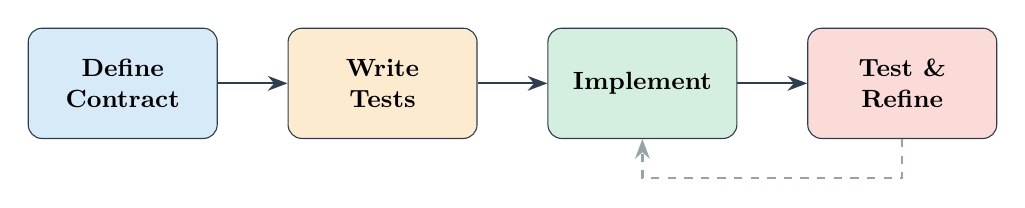
\begin{tikzpicture}[
    stage/.style={rectangle, rounded corners=5pt, draw=csprimary, fill=#1, minimum width=24mm, minimum height=14mm, font=\small\bfseries, align=center},
    arrow/.style={-{Stealth[length=2.5mm]}, thick, color=csprimary}
]

\node[stage=cstertiary!20] (define) at (0,0) {Define\\Contract};
\node[stage=cswarm!20] (test) at (3.3,0) {Write\\Tests};
\node[stage=csaccent!20] (impl) at (6.6,0) {Implement};
\node[stage=cssecondary!20] (verify) at (9.9,0) {Test \&\\Refine};

\draw[arrow] (define) -- (test);
\draw[arrow] (test) -- (impl);
\draw[arrow] (impl) -- (verify);

% Feedback loop
\draw[arrow, dashed, color=codegray] (verify.south) -- ++(0,-0.5) -| (impl.south);

\end{tikzpicture}
\end{center}

%---------- PRINCIPLES ----------%
\section{Principles of Good Functions}

Across all our famous functions, certain principles emerge:

\textbf{Do one thing well.} A function should have a single, clear purpose. If you can't describe what a function does in one sentence, it's probably doing too much.

\textbf{Use meaningful names.} \texttt{hypotenuse()} is better than \texttt{calc()}. \texttt{linearSearch()} tells you exactly what algorithm is used. Names are documentation.

\textbf{Handle edge cases.} What happens with empty input? Zero? Negative numbers? The quadratic formula handles the case of no real solutions; factorial handles 0 and 1. Anticipate the unusual.

\textbf{Document your assumptions.} Binary search \textit{requires} a sorted array. If your function has preconditions, state them clearly in comments.

\textbf{Prefer clarity over cleverness.} Code is read far more often than it's written. A simple, obvious implementation beats a clever, confusing one---even if the clever version is slightly faster.

The functions we've explored have endured because they're not just correct---they're clear, well-defined, and focused. These qualities matter whether you're implementing ancient mathematics or inventing something new.

%---------- DISCUSSION QUESTIONS ----------%
\section*{Discussion Questions}

\begin{questionbox}
\begin{enumerate}[leftmargin=*, label=\textcolor{cswarm}{\textbf{\arabic*.}}]
    \item \textbf{Iteration vs.\ Recursion:} We saw both iterative and recursive implementations of factorial. What are the advantages of each approach? When might you prefer one over the other? Are there problems that are more naturally expressed recursively?

    \item \textbf{The Sorted Requirement:} Binary search only works on sorted data. In what situations would it be worth sorting an array just to use binary search? When would linear search be preferable despite being slower?

    \item \textbf{Edge Cases:} The quadratic formula must handle three cases (two solutions, one, or none). What would happen if we didn't check the discriminant and just applied the formula blindly? Why is handling edge cases important?

    \item \textbf{Historical Algorithms:} Many algorithms we use today were discovered centuries or millennia ago. Why do you think these mathematical insights have remained useful? What does it suggest about the nature of mathematical truth?

    \item \textbf{Testing Challenges:} How would you test the \texttt{binarySearch} function thoroughly? What inputs would you try? How many test cases are ``enough''? Is it possible to prove a function is correct through testing alone?
\end{enumerate}
\end{questionbox}

%---------- GLOSSARY ----------%
\section*{Key Terms}

\begin{glossarybox}
\begin{description}[leftmargin=!, labelwidth=3.2cm, font=\bfseries\color{cssecondary}]
    \item[Base Case] In recursion, the condition that stops the function from calling itself, providing a direct answer.
    
    \item[Binary Search] A search algorithm for sorted arrays that repeatedly halves the search space, achieving O(log n) time.
    
    \item[Discriminant] In the quadratic formula, the expression $b^2 - 4ac$ that determines the number of real solutions.
    
    \item[Factorial] The product of all positive integers up to $n$, written $n!$, fundamental to counting and probability.
    
    \item[Function] A reusable block of code that takes inputs (parameters), performs a task, and returns an output.
    
    \item[Javadoc] A documentation format for Java using special comments (\texttt{/** */}) to describe functions, parameters, and return values.
    
    \item[Linear Search] A search algorithm that checks each element sequentially, working on any array but taking O(n) time.
    
    \item[O(log n)] Logarithmic time complexity, where the time grows with the logarithm of the input size---very efficient.
    
    \item[O(n)] Linear time complexity, where the time grows proportionally with the input size.
    
    \item[Parameter] A variable in a function definition that receives a value when the function is called.
    
    \item[Pythagorean Theorem] The relation $a^2 + b^2 = c^2$ for right triangles, used to calculate distances.
    
    \item[Quadratic Equation] An equation of the form $ax^2 + bx + c = 0$, solved by the quadratic formula.
    
    \item[Recursion] A technique where a function calls itself to solve smaller instances of the same problem.
    
    \item[Return Type] The data type of the value a function produces, declared before the function name.
    
    \item[Signature] The function's name, return type, and parameter list---its external interface.
    
    \item[Test-Driven Development] A practice of writing test cases before implementing the code they test.
\end{description}
\end{glossarybox}

\vspace{5mm}

%---------- FOOTER ----------%
\begin{center}
\textcolor{csprimary}{\rule{0.6\textwidth}{0.5pt}}\\[3mm]
{\small\textcolor{gray}{This case study is part of the Open Educational Resources for \cscourse.\\
Licensed under Creative Commons Attribution 4.0 (CC BY 4.0).}}
\end{center}

\end{document}